\ifx\allfiles\undefined
\documentclass[12pt, a4paper, oneside, UTF8]{ctexbook}  %  这一句是新增加的
\usepackage[dvipsnames]{xcolor}
\usepackage{amsmath}   % 数学公式
\usetikzlibrary{arrows, calc, decorations.pathmorphing}
\newcommand{\pa}{\partial}
\newcommand{\vvec}{\overset{\rightharpoonup\!\!\!\! \rightharpoonup}}


\begin{document}
%\title{\Huge{\textbf{赵爹《连续介质力学》笔记}}}
\author{作者:无名氏马}
\date{\today}
\maketitle                   % 在单独的标题页上生成一个标题

\thispagestyle{empty}        % 前言页面不使用页码
\begin{center}
    \Huge\textbf{前言}
\end{center}

    本笔记根据
    \href{https://www.bilibili.com/video/BV1c54y1W78q/?spm_id_from=333.1387.upload.video_card.click&vd_source=0745441b4a83ceba73d32af3b7b0a955}{赵亚溥老师2020年春季《连续介质力学》课程}
    和教材
    (赵亚溥. 理性力学教程. 北京: 科学出版社, 2020.)整理而成,仅供参考学习。

\begin{flushright}
    \begin{tabular}{c}
        \today
    \end{tabular}
\end{flushright}

\newpage                      % 新的一页
\pagestyle{plain}             % 设置页眉和页脚的排版方式(plain:页眉是空的,页脚只包含一个居中的页码)
\setcounter{page}{1}          % 重新定义页码从第一页开始
\pagenumbering{Roman}         % 使用大写的罗马数字作为页码
\tableofcontents              % 生成目录

\newpage                      % 以下是正文
\pagestyle{plain}
\setcounter{page}{1}          % 使用阿拉伯数字作为页码
\pagenumbering{arabic}
% \setcounter{chapter}{-1}    % 设置 -1 可作为第零章绪论从第零章开始
 % 单独编译时,其实不用编译封面目录之类的,如需要不注释这句即可
\else
\fi
%  ↓↓↓↓↓↓↓↓↓↓↓↓↓↓↓↓↓↓↓↓↓↓↓↓↓↓↓↓ 正文部分
\chapter{张量运算}
\section{class 27}
\begin{proposition}
    \[
    \vvec{A}:\left(\vvec{B}\vvec{C}\right)
    =\left(\vvec{B^T}\vvec{A}\right):\vvec{C}
    =\left(\vvec{A}\vvec{C^T}\right):\vvec{B}\]
\end{proposition}
\begin{proposition}
    Taylor expansion of scalar function of tensor
    \[
    \psi\left(\vvec{A}+d\vvec{A}\right)=\psi\left(\vvec{A}\right)
    +\frac{\pa \psi}{\pa \vvec{A}}:\vvec{A}+o\left(d\vvec{A}\right)\]
    \[
        \psi\left(\vvec{A}+\alpha\vvec{B}\right)=\psi\left(\vvec{A}\right)
        +\alpha\frac{\pa \psi}{\pa \vvec{A}}:\vvec{B}+o\left(\alpha\vvec{B}\right)
    \]
\end{proposition}
\begin{defn}
    time derivative
\begin{gather*}
        \frac{d}{dt}\left(\vvec{A^{-1}}\right)=\dot{\vvec{A^{-1}}}\\
        \vvec{A^{-1}}\vvec{A}=\vvec{I},\dot{\vvec{A^{-1}}\vvec{A}}=\vvec0\\
        \dot{\vvec{A^{-1}}}\vvec{A}+\vvec{A^{-1}}\dot{\vvec{A}}=0\\
        \dot{\vvec{A^{-1}}}=-\vvec{A^{-1}}\dot{\vvec{A}}\vvec{A^{-1}}
\end{gather*}
\end{defn}
\begin{defn}
    differentiation of a scalar function
    \begin{align*}
        \frac{\pa \psi}{\pa \vvec{A}}:\vvec{B}&=\lim_{\alpha\rightarrow0}
        \frac{\psi\left(\vvec{A}+\alpha\vvec{B}\right)-\psi\left(\vvec{A}\right)}{\alpha}\\
        &=\frac{d\psi\left(\vvec{A}+\alpha\vvec{B}\right)}{d\alpha}|_{\alpha=0}
    \end{align*}
\end{defn}
\begin{example}
    \begin{gather*}
        \frac{\pa tr\vvec{A}}{\pa\vvec{A}}:\vvec{B}
        =\lim_{\alpha\rightarrow0}\frac{\vvec{I}:\left(\vvec{A}+\alpha\vvec{B}\right)
        -\vvec{I}:\vvec{A}}{\alpha}=\vvec{I}:\vvec{B}\\
        \frac{\pa tr\vvec{A}}{\pa\vvec{A}}=\vvec{I}
    \end{gather*}
    \begin{align*}        
        &\frac{\pa tr\left(\vvec{A^2}\right)}{\pa\vvec{A}}
        =\frac{\pa tr\left(\vvec{A}\vvec{A}\right)}{\pa\vvec{A}}
        =\frac{\pa \vvec{A^T}\vvec{A}}{\pa\vvec{A}}\\
        \frac{\pa tr\vvec{A^2}}{\pa\vvec{A}}:\vvec{B}
        &=\lim_{\alpha\rightarrow0}\frac{\left(\vvec{A}+\alpha\vvec{B}\right)^T:
        \left(\vvec{A}+\alpha\vvec{B}\right)-\vvec{A^T}:\vvec{A}}{\alpha}\\
        &=\vvec{B^T}:\vvec{A}+\vvec{A^T}:\vvec{B}
        +\lim_{\alpha\rightarrow0}\alpha\vvec{B^T}\vvec{B}\\
        &=\left(\vvec{I}\vvec{B^T}\right):\vvec{A}
        +\vvec{A^T}:\vvec{B}+0\\
        &=2\vvec{A^T}:\vvec{B}        
    \end{align*}
    \[\frac{\pa tr\left(\vvec{A^n}\right)}{\pa\vvec{A}}
    =n\left(\vvec{A^{n-1}}\right)^T\]
\end{example}
\begin{example}
    \[
    \vvec{I}:\left(\vvec{A}\vvec{B}+\vvec{B}\vvec{A}\right)
    =\vvec{I}:\left(2\vvec{A}\vvec{B}\right)
    =2\vvec{A^T}:\vvec{B}
    \]
\end{example}
\begin{add}    
    对于一个二阶张量 \( \vvec{T} \),其不变量可以通过以下公式计算:
    
    1. 第一不变量(迹):
    \[
    I_1 = \text{tr}(\vvec{T}) = T_{ii}
    \]
    
    2. 第二不变量:
    \[
    I_2 = \frac{1}{2} \left[ (\text{tr}(\vvec{T}))^2 - \text{tr}(\vvec{T^2}) \right] = \frac{1}{2} \left( T_{ii} T_{jj} - T_{ij} T_{ji} \right)
    \]
    
    3. 第三不变量(行列式):
    \[
    I_3 = \det(\vvec{T}) = \epsilon_{ijk} T_{1i} T_{2j} T_{3k}
    \]
    
    其中,\( T_{ij} \) 是张量 \( \vvec{T} \) 的分量,\( \epsilon_{ijk} \) 是 Levi-Civita 符号。
\end{add}
\begin{corollary}
    \[tr\vvec{S^2}=\vvec{I}:\vvec{S^2}=\vvec{S^T}:\vvec{S}
    =\left(S_{ij}\vec{e_j}\otimes\vec{e_i}\right):\left(S_{kl}\vec{e_k}\otimes\vec{e_l}\right)
    =S_{ij}S_{kl}\delta_{jk}\delta_{il}=S_{ij}S_{ji}=I_1^2\]
    \begin{align*}
        \text{tr} \vvec{S^3}&= \vvec{I} : \vvec{S^3} = \vvec{S^T} : \vvec{S^2} 
        =S_{ij} S_{jk} S_{kl} \, \vec{e}_i \otimes \vec{e}_l
        =S_{ij} S_{jk} S_{ki}=I_1^3\\
        &=S_{11}^3 + S_{22}^3 + S_{33}^3 
        + 3 S_{11} S_{12} S_{21} + 3 S_{11} S_{13} S_{31} \\
        &\quad + 3 S_{22} S_{21} S_{12} + 3 S_{22} S_{23} S_{32} 
        + 3 S_{33} S_{31} S_{13} + 3 S_{33} S_{32} S_{23} \\
        &\quad + 6 S_{11} S_{22} S_{33}
        \end{align*}    
    \begin{align*}
        \left(tr\vvec{S}\right)^2&=\left(S_{11} + S_{22} + S_{33}\right)^2 \\
        &= S_{11}^2 + S_{22}^2 + S_{33}^2 
         + 2 S_{11} S_{22} + 2 S_{11} S_{33} + 2 S_{22} S_{33}\\
        &=S_{ii}S_{jj}=I_1^2 - 2 I_2
    \end{align*}
    \begin{align*}
        \left(tr\vvec{S}\right)^3         
        &=S_{11}^3 + S_{22}^3 + S_{33}^3 
        + 3 S_{11}^2 S_{22} + 3 S_{11}^2 S_{33} \\
        &\quad + 3 S_{22}^2 S_{11} + 3 S_{22}^2 S_{33} 
        + 3 S_{33}^2 S_{11} + 3 S_{33}^2 S_{22} \\
        &\quad + 6 S_{11} S_{22} S_{33}\\
        &=S_{ii} S_{jj} S_{kk}=I_1^3 - 3 I_1 I_2 + 3 I_3
    \end{align*}
\end{corollary}
\begin{defn}
    张量不变量的导数
\[\begin{cases}
\frac{\partial I_1(\vvec{A})}{\partial \vvec{A}} = \frac{\partial \text{tr}\vvec{A}}{\partial \vvec{A}} = I \\
\frac{\partial I_2(\vvec{A})}{\partial \vvec{A}} = \frac{1}{2}\left(\frac{\partial (\text{tr}\vvec{A})^2}{\partial \vvec{A}} - \frac{\partial \text{tr}\vvec{A^2}}{\partial \vvec{A}}\right) = I_1I - \vvec{A^T} \\
\frac{\partial I_3(\vvec{A})}{\partial \vvec{A}} = \frac{1}{6}\left(\frac{\partial (\text{tr}\vvec{A})^3}{\partial \vvec{A}} - 3\frac{\partial}{\partial \vvec{A}}\left((\text{tr}\vvec{A})(\text{tr}\vvec{A^2})\right) 
+ 2\frac{\partial \text{tr}\vvec{A^3}}{\partial \vvec{A}}\right) = (\vvec{A^T})^2 - I_1\vvec{A^T} + I_2\vvec{I}
\end{cases}\]

考虑到 \( I_3(\vvec{A}) = \det \vvec{A} \),以及 \( (\vvec{A^T})^2 - I_1\vvec{A^T} + I_2\vvec{I} = I_3\vvec{A^{-T}} \),亦即
\[
\frac{\partial \det \vvec{A}}{\partial \vvec{A}} = (\det \vvec{A})\vvec{A^{-T}} = \text{Cof}\vvec{A}
\]

式中,\(\text{Cof}\vvec{A}\) 为 \( \vvec{A} \) 的余子式矩阵(cofactor matrix)。

如果令 \( \vvec{A} \) 为变形梯度张量 \( \vvec{F} \),则有如下常用关系式:
\[
\frac{\partial \det \vvec{F}}{\partial \vvec{F}} = \frac{\partial J}{\partial \vvec{F}} = (\det \vvec{F})\vvec{F^{-T}} = J\vvec{F^{-T}} = \text{Cof}\vvec{F}
\]
\end{defn}
\section{class 28}
\begin{add}
    旋转李群——SO(n)和SU(n)\textbf{(摘自教材)}

物理学与各种旋转结下不解之缘,从力学中研究的刚体转动,到量子理论中的粒子自旋。地球绕太阳转,月亮绕地球转,滚珠在轴承滚道中转,电子绕原子核转,每一层次的实验和理论中似乎都少不了旋转。物理中的旋转除了在真实时空中的旋转之外,还有一大部分是在假想的、抽象的空间中的旋转,比如动量空间,希尔伯特空间,自旋空间,同位旋空间等。

空间中的旋转也构成群,并且,旋转群(rotation group)是物理中非常重要的一类群。旋转群有离散的和连续的之分。连续旋转群具有天然的流形结构,是一种李群,理论物理,特别是统一理论中所感兴趣的旋转李群有 \(SO(3)\)、\(SO(2)\)、\(U(1)\)、\(SU(2)\)、\(SU(3)\) 等。

旋转可以用大家熟知的矩阵来表示。因此,我们首先用矩阵的语言,解释一下上面所列的一串符号是什么意思:括号中的数目字(3, 2, 1)等是表示旋转的矩阵空间的维数;大写字母 O 代表正交矩阵(orthogonal matrix);U 代表酉矩阵(unitary matrix);S 是特殊的(special)意思,表示矩阵的行列式为 1。

比如,举三维空间的旋转群 \(O(3)\) 为例。此处 3 是指旋转空间的维数,O 对应于保持长度和角度不变的正交变换矩阵。具体一点说,正交矩阵 \(O(3)\) 是一个由 \(3 \times 3 = 9\) 个实数组成的矩阵,它的三个列向量或者三个行向量,都构成三维空间中三个正交的单位矢量。一般来说,正交矩阵 \(O(3)\) 的行列式可为 1 或 -1。当行列式为 -1 时,正交矩阵表示的变换是旋转再加反演,这里的负号便来自反演。上述的 \(O(3)\) 旋转群如果加上字母 S,指的便是特殊旋转群 \(SO(3)\),那意味着,矩阵行列式被限制为 1。所以,\(SO(3)\) 表示的是三维空间中无反演的纯粹旋转。

观察我们周围的世界:人的左脸并不完全等同于右脸;大多数人的心脏长在左边,大多数的 DNA 分子是右旋的;地球并不是一个完全规则的球形……正是因为对称中有了这些不对称的元素,对称与不对称的和谐交汇,创造了我们的世界。

\begin{figure}[h]
\centering
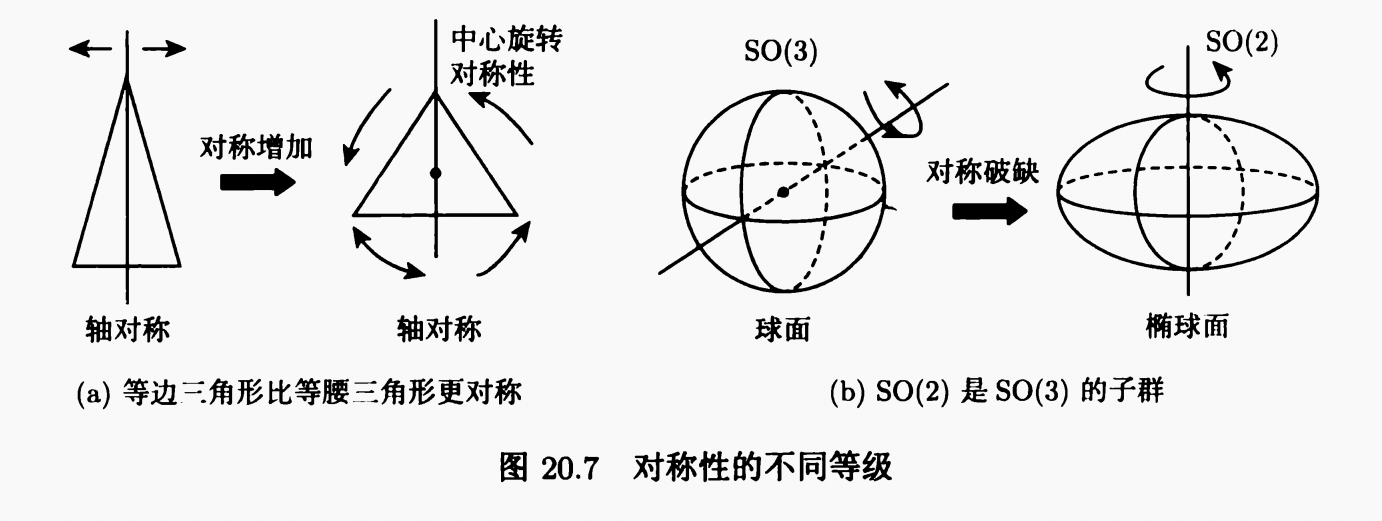
\includegraphics[width=0.7\textwidth, keepaspectratio]{chap4/20.7.png}
\label{image20.7}
\end{figure}

不妨深究一下,何谓对称?何谓不对称?可以说,对称中有不对称,不对称中又有对称。并且,对称有多种多样,就几何图像而言,具有某种变换下的对称,但对另一种变换便可能不对称。即使是同一类型的对称,也有对称程度的高低。比如说,一个正三角形,和一个等腰三角形比较,正三角形应该更为对称一些,如图 20.7(a)。再举旋转群为例:一个球面是三维旋转对称的,在 \(SO(3)\) 群作用下不变,而椭球面只能看作是在二维旋转群 \(SO(2)\) 的作用下不变了。用不很严格地说法,\(SO(2)\) 是 \(SO(3)\) 的子群。因此,球面比椭球面具有更多的对称性。如果从对称性的高低等级来定义的话,系统从对称性高的状态,演化到对称性更低的状态,被称为“对称破缺”,反之,则可称为“对称建立”。例如,当正三角形变形为等腰三角形,或者当球面变成椭球面,我们便说“对称破缺了”。从李群的观点来看,\(SO(3)\) 是三阶的,有三个生成元。\(SO(2)\) 只有一个生成元,从球面到椭球面,两个对称性被破缺。因此,可以从群论的观点来研究对称破缺。
\end{add}
\begin{defn}
    electromagnetic tensor
    
    国际单位制中的一种矩阵形式
\[F^{\mu\nu} = -F^{\nu\mu}=
\begin{pmatrix}
0 & -E_x/c & -E_y/c & -E_z/c \\
E_x/c & 0 & -B_z & B_y \\
E_y/c & B_z & 0 & -B_x \\
E_z/c & -B_y & B_x & 0
\end{pmatrix}
\]

另一种矩阵形式,略去系数
\[F_{\mu\nu} = -F_{\nu\mu}=
\begin{pmatrix}
    0 & E_x & E_y & E_z \\
    -E_x & 0 & -B_z & B_y \\
    -E_y & B_z & 0 & -B_x \\
    -E_z & -B_y & B_x & 0
    \end{pmatrix}
    \]    
\end{defn}
\begin{defn}
    Cayley\textminus Hamilton theorem
    \[\boxed{\vvec{S}^3-I_1\vvec{S}^2+I_2\vvec{S}-I_3=\vvec{0}}\]
    \begin{tui}
        \[\vvec{S}\vec{v}=\lambda\vec{v}\Rightarrow\left(\vvec{S}-\lambda\vvec{I}\right)\vec{v}=\vec{0}\]
        
        homogeneous equations
\begin{align*}
    \det\left(\vvec{S}-\lambda\vvec{I}\right)=0&\Rightarrow
    \lambda^3-I_1\lambda^2+I_2\lambda-I_3=\vec{0}\\
    &\Rightarrow\vvec{S}^3-I_1\vvec{S}^2+I_2\vvec{S}-I_3=\vvec{0}
\end{align*}
    \end{tui}
\end{defn}
\begin{lemma}
    \[\det\left(\vvec{S}-\lambda\vvec{I}\right)=0\Rightarrow
    \lambda^3-I_1\lambda^2+I_2\lambda-I_3=0\]
    \begin{tui}
        给定一个二阶张量 \(\vvec{S}\),其特征方程为:
        \[
        \det\left(\vvec{S} - \lambda \vvec{I}\right) = 0
        \]
        
        其中,\(\lambda\) 是特征值,\(\vvec{I}\) 是单位张量。
        
        展开行列式:
        \[
        \det\left(\vvec{S} - \lambda \vvec{I}\right) = 
        \begin{vmatrix}
        S_{11} - \lambda & S_{12} & S_{13} \\
        S_{21} & S_{22} - \lambda & S_{23} \\
        S_{31} & S_{32} & S_{33} - \lambda
        \end{vmatrix}
        \]
        
        使用行列式的展开公式,沿第一行展开:
        \begin{align*}
        &\quad\det\left(\vvec{S} - \lambda \vvec{I}\right)\\
        &= (S_{11} - \lambda) \cdot 
        \begin{vmatrix}
        S_{22} - \lambda & S_{23} \\
        S_{32} & S_{33} - \lambda
        \end{vmatrix} 
        \quad - S_{12} \cdot 
        \begin{vmatrix}
        S_{21} & S_{23} \\
        S_{31} & S_{33} - \lambda
        \end{vmatrix} 
        \quad + S_{13} \cdot 
        \begin{vmatrix}
        S_{21} & S_{22} - \lambda \\
        S_{31} & S_{32}
        \end{vmatrix}\\
        &=(S_{11} - \lambda) \left[ (S_{22} - \lambda)(S_{33} - \lambda) - S_{23} S_{32} \right] \\
        &\quad - S_{12} \left[ S_{21} (S_{33} - \lambda) - S_{23} S_{31} \right] 
         + S_{13} \left[ S_{21} S_{32} - (S_{22} - \lambda) S_{31} \right]\\
        &=(S_{11} - \lambda)(S_{22} - \lambda)(S_{33} - \lambda)
         - (S_{11} - \lambda) S_{23} S_{32} \\
        &\quad - S_{12} S_{21} (S_{33} - \lambda) + S_{12} S_{23} S_{31} 
        + S_{13} S_{21} S_{32} - S_{13} (S_{22} - \lambda) S_{31}\\
        &=(S_{11} S_{22} S_{33}) 
        - \lambda (S_{11} S_{22} + S_{11} S_{33} + S_{22} S_{33}) 
        + \lambda^2 (S_{11} + S_{22} + S_{33})  - \lambda^3 \\
        &\quad+ \text{其他项(涉及非对角元素的乘积)}\\
        &=\lambda^3 - I_1 \lambda^2 + I_2 \lambda - I_3
        \end{align*}
        \end{tui}
\end{lemma}
\begin{example}
由Cayley-Hamilton定理推导出二阶张量第三主不变量 \(I_3\)
\begin{yzh}
\begin{gather*}  
        I_1 = \text{tr}(\vvec{T}) = T_{ii}\\
        I_2 = \frac{1}{2} \left[ (\text{tr}(\vvec{T}))^2 - \text{tr}(\vvec{T^2}) \right] = \frac{1}{2} \left( T_{ii} T_{jj} - T_{ij} T_{ji} \right)
\end{gather*} 
\end{yzh}
\begin{tui}
根据Cayley-Hamilton定理,一个二阶张量 \(\vvec{T}\) 满足其自身的特征方程:

\[
\vvec{T^3} - I_1 \vvec{T^2} + I_2 \vvec{T} - I_3 \vvec{I} = \vvec{0}
\]

为了推导出第三主不变量 \(I_3\),我们可以对上述方程取迹(trace)。迹运算具有线性性质,且 \(\text{tr}(\vvec{I}) = 3\),因此:

\[
\text{tr}(\vvec{T^3}) - I_1 \text{tr}(\vvec{T^2}) + I_2 \text{tr}(\vvec{T}) - I_3 \text{tr}(\vvec{I}) = 0
\]

将 \(\text{tr}(\vvec{I}) = 3\) 代入上式,
并将方程整理为关于 \(I_3\) 的形式:
\[
I_3 = \frac{1}{3} \left( \text{tr}(\vvec{T^3}) - I_1 \text{tr}(\vvec{T^2}) + I_2 \text{tr}(\vvec{T}) \right)
\]

进一步代入 \(I_1\) 和 \(I_2\) 的表达式:
\begin{align*}
I_3 &= \frac{1}{3} \left( \text{tr}(\vvec{T^3}) - \text{tr}(\vvec{T}) \text{tr}(\vvec{T^2}) 
+ \frac{1}{2} \left( (\text{tr}(\vvec{T}))^2 - \text{tr}(\vvec{T^2}) \right) \text{tr}(\vvec{T}) \right)\\
 &= \frac{1}{6}\left(2\text{tr}(\vvec{T^3})+(\text{tr}(\vvec{T}))^3
 -3\text{tr}(\vvec{T^2})\text{tr}(\vvec{T})\right)  
\end{align*}
\end{tui}
\end{example}
\section{class 29}
\begin{defn}
    \[\frac{\pa \det\vvec{A}}{\pa\vvec{A}}=\frac{\pa I_3(\vvec{A})}{\pa\vvec{A}}=?\]
    \begin{align*}
        \det\left(\vvec{A}+\lambda\vvec{I}\right)
        &=\lambda^3 + I_1 \lambda^2 + I_2 \lambda + I_3\\
        \frac{\pa \det\vvec{A}}{\pa\vvec{A}}:\vvec{B}
        &=\lim_{\alpha\rightarrow0}\frac{\det\left(\vvec{A}+\alpha\vvec{B}\right)
        -\det\vvec{A}}{\alpha}\\
        &=\lim_{\alpha\rightarrow0}\frac{\det\left(\alpha\vvec{A}(\alpha^{-1}\vvec{A}+\vvec{A^{-1}}\vvec{B})\right)
        -\det\vvec{A}}{\alpha}\\
        \because\quad\det\left(\alpha\vvec{A}(\alpha^{-1}\vvec{A}+\vvec{A^{-1}}\vvec{B})\right)
        &=\left(\alpha^3\det\vvec{A}\right)\underbrace{\det\left(\alpha^{-1}\vvec{A}+\vvec{A^{-1}}\vvec{B}\right)}\\
        \det\left(\alpha^{-1}\vvec{A}+\vvec{A^{-1}}\vvec{B}\right)&=\alpha^{-3} + I_1(\vvec{A^{-1}}\vvec{B}) \alpha^{-2} 
        + I_2(\vvec{A^{-1}}\vvec{B}) \alpha^{-1} + I_3(\vvec{A^{-1}}\vvec{B})
    \end{align*}
    \begin{align*}
        \frac{\pa \det\vvec{A}}{\pa\vvec{A}}:\vvec{B}
        &=\lim_{\alpha\rightarrow0}\frac{\det\vvec{A}-\det\vvec{A}+I_1(\vvec{A^{-1}}\vvec{B}) \alpha\det\vvec{A} 
        +\alpha^2\dots + \alpha^3\dots}{\alpha}\\
        &=I_1(\vvec{A^{-1}}\vvec{B}) \det\vvec{A}=\left(\vvec{I}:(\vvec{A^{-1}}\vvec{B}) \right)\det\vvec{A}\\
        &=\left(\vvec{A^{-T}}:\vvec{B}\right)\det\vvec{A}
    \end{align*}
    \[\boxed{\frac{\pa \det\vvec{A}}{\pa\vvec{A}}=\det\vvec{A}\vvec{A^{-T}}}\]
\end{defn}
\begin{corollary}
    \[\frac{\pa J^{-1}}{\pa\vvec{A}}=-J^{-1}\vvec{A^{-T}}\]
    \[\boxed{\frac{\pa J^{-n}}{\pa\vvec{A}}=-nJ^{-n}\vvec{A^{-T}}}\]
    \begin{proof}
        \begin{gather*}
            \frac{\pa J^{-1}}{\pa\vvec{A}}=\frac{\pa \det\vvec{A}}{\pa\vvec{A}}
            =J^{-1}\vvec{A^{-T}}\\
            \frac{\pa J^{-1}}{\pa\vvec{A}}=\frac{\pa J^{-1}}{\pa J}\frac{\pa J}{\pa\vvec{A}}
            =-J^{-2}J^{-1}\vvec{A^{-T}}=-J^{-1}\vvec{A^{-T}}
        \end{gather*}
    \end{proof}
\end{corollary}
\begin{defn}
    四阶单位张量

    用空芯正体符号 $\mathbb{I}$ 表示的四阶单位张量 (fourth-order identity tensor) 定义为
    \[
    \mathbb{I} = \delta_{ik}\delta_{jl}\vec{e_i} \otimes \vec{e_j} \otimes \vec{e_k} \otimes \vec{e_l}
    \]
    
    与两个二阶单位张量 $\vvec{I} = \delta_{ij}\vec{e_i} \otimes \vec{e_j}$ 的并矢为
    \[
    \vvec{I} \otimes \vvec{I} = \delta_{ij}\delta_{kl}\vec{e_i} \otimes \vec{e_j} \otimes \vec{e_k} \otimes \vec{e_l}
    \]

    不同

    四阶单位张量的性质
    \begin{align*}
\mathbb{I}: \vvec{A}& = (\delta_{ik}\delta_{jl}\vec{e_i} \otimes \vec{e_j} \otimes \vec{e_k} \otimes \vec{e_l}) : (A_{op}e_o \otimes e_p) = \delta_{ik}\delta_{jl}\delta_{ko}\delta_{lp}A_{op}\vec{e_i} \otimes \vec{e_j}\\
&= \delta_{ik}\delta_{ko}\delta_{jl}\delta_{lp}A_{op}\vec{e_i} \otimes \vec{e_j} = \delta_{io}\delta_{jp}A_{op}\vec{e_i} \otimes \vec{e_j} = A_{op}e_o \otimes e_p = \vvec{A}
    \end{align*}
\end{defn}
\begin{defn}
    对称的四阶单位张量
\[
\mathbb{I}^T = \delta_{jk} \delta_{il} \vec{e_i} \otimes \vec{e_j}\otimes \vec{e_k} \otimes \vec{e_l}  \Leftrightarrow  \mathbb{I}^T : \vvec{A} = \vvec{A^T}
\]

上式,就是四阶单位张量的转置,亦可写为
\[
\mathbb{I}^T = \vec{e_i} \otimes \vec{e_j} \otimes \vec{e_j} \otimes \vec{e_i}
\]

四阶单位张量和其转置可组成对称的四阶单位张量 (symmetrical fourth-order identity tensor):
\[
\mathbb{I}^s = \frac{\mathbb{I} + \mathbb{I}^T}{2} = \frac{1}{2} (\delta_{ik} \delta_{jl} + \delta_{jk} \delta_{il}) \vec{e_i} \otimes \vec{e_j} \otimes \vec{e_k} \otimes \vec{e_l}
\]

对称的四阶单位张量的性质

minor Symmetry
\[
\mathbb{I}_{ijkl}^s = \mathbb{I}_{jikl}^s, \quad \mathbb{I}_{ijkl}^s = \mathbb{I}_{ijlk}^s
\]

major symmetries
\[
\mathbb{I}_{ijkl}^s = \mathbb{I}_{klij}^s
\]

对于任意一个对称的二阶张量 $\vvec{A}$ 满足:
\[
\frac{\partial \vvec{A}}{\partial \vvec{A}} = \mathbb{I}^s
\]
\end{defn}
\begin{defn}
    四阶投影张量

    一个任意的二阶张量 $\vvec{A}$ 可分解为球形分量 (spherical part) 和偏量 (deviatoric part):
\[
\vvec{A} = \underbrace{\alpha \vvec{I}}_{\text{球量}} + \underbrace{dev \vvec{A}}_{\text{偏量}}
\]

由于偏量部分是无迹的(traceless),对上述式求迹,有
\[
\alpha = \frac{1}{3}tr\vvec{A} = \frac{1}{3}(\vvec{I}:\vvec{A})
\]

则二阶张量 $\vvec{A}$ 的偏量 $dev\vvec{A}$ 可通过四阶单位张量 $\mathbb{I}$ 表示为
\begin{align*}
dev\vvec{A} &= \vvec{A} - \frac{1}{3}\vvec{I}(\vvec{I}:\vvec{A}) = \vvec{A} - \frac{1}{3}(\vvec{I}\otimes \vvec{I}):\vvec{A}\\
& = \left[ \mathbb{I} - \frac{1}{3}(\vvec{I}\otimes \vvec{I}) \right]:\vvec{A}= \mathbb{P}:\vvec{A}
\end{align*}

式中,四阶投影张量为
\[
\mathbb{P} = \mathbb{I} - \frac{1}{3}(\vvec{I}\otimes \vvec{I})
\]
\end{defn}
\begin{example}
    主应力张量$\vvec{A}$
    \[
    dev\vvec{A}=\begin{vmatrix}
        \sigma_1-\frac{\sigma_1+\sigma_2+\sigma_3}{3} & & \\
         &\sigma_2-\frac{\sigma_1+\sigma_2+\sigma_3}{3} & \\
         & &\sigma_3-\frac{\sigma_1+\sigma_2+\sigma_3}{3} 
    \end{vmatrix}
    \]
    
    静水压强
    \[
        \begin{vmatrix}
            S_1 & & \\
             &S_2 & \\
             & &S_3 
        \end{vmatrix}=\begin{vmatrix}
            \sigma_1-\sigma_m & & \\
             &\sigma_2-\sigma_m& \\
             & &\sigma_3-\sigma_m
        \end{vmatrix},\sigma_m=\frac{\sigma_1+\sigma_2+\sigma_3}{3}
    \]
    
    偏量的特征方程\(\vvec{S}^3-I_1\vvec{S}^2+I_2\vvec{S}-I_3=\vvec{0}\)
    \[
    \begin{cases}  
            I_1 = S_1+S_2+S_3=0\\
            I_2 = -\left( S_1S_2+S_2S_3+S_3S_1 \right)\\
            \,\quad=-(\sigma_1-\sigma_m)(\sigma_2-\sigma_m)
            -(\sigma_2-\sigma_m)(\sigma_3-\sigma_m)-(\sigma_3-\sigma_m)(\sigma_1-\sigma_m)
            \\\,\quad=2(\sigma_1+\sigma_2+\sigma_3)\sigma_m-3\sigma_m^2
            -(\sigma_1\sigma_2+\sigma_2\sigma_3+\sigma_3\sigma_1)
            \\\,\quad=\frac{1}{6}\left[(\sigma_1-\sigma_2)^2+(\sigma_2-\sigma_3)^2+(\sigma_3-\sigma_1)^2\right]
            \\I_3 = S_1S_2S_3
    \end{cases}
    \]
\end{example}
\section{class 30}
\begin{defn}
    谱定理(spectral theorem)

    若 $\vvec{S}$ 是对称张量,则存在线性空间 $\mathcal{V}$ 中的一个标准正交基,它完全由 $\vvec{S}$ 的本征向量组成。此外,对于一个这样的基 $\vec{e}_1, \vec{e}_2, \vec{e}_3$ 按次序排列的相应的本征值 $\omega_1, \omega_2, \omega_3$ 构成 $\vvec{S}$ 的整个谱,且
    \[
    \vvec{S} = \sum_i \omega_i \vec{e}_i \otimes \vec{e}_i
    \tag{30-1}
    \]

    反之,如果 $\vvec{S}$ 具有形式 (30-1),其中 $\{\vec{e}_i\}$ 是标准正交的,则 $\omega_1, \omega_2, \omega_3$ 是相对应于本征向量 $\vec{e}_1, \vec{e}_2, \vec{e}_3$ 的本征值。此外:
    
    (a) 当且仅当 $\vvec{S}$ 的本征空间是通过0的三个互相垂直的直线时,$\vvec{S}$ 恰好有三个不同的本征值,且 $\vvec{S}$ 表示为 $\vvec{S} = \omega_1 \vec{e}_1 \otimes \vec{e}_1 + \omega_2 \vec{e}_2 \otimes \vec{e}_2 + \omega_3 \vec{e}_3 \otimes \vec{e}_3$;
\begin{flushleft}
    \begin{minipage}[t]{0.7\textwidth}
        \vspace{0pt}
        \raggedright 
    (b) 当且仅当 $\vvec{S}$ 有两个不同的本征值 $\omega_1$ 和 $\omega_2$,其对应的本征空间分别是一条通过0的线l以及通过0并垂直于l的平面(如图13.1所示),则 $\vvec{S}$ 表示为
    \[
        \vvec{S} = \omega_1 \vec{e} \otimes \vec{e} + \omega_2 (\vvec{I} - \vec{e} \otimes \vec{e})
        \tag{30-2}
    \]
           
    反之,当且仅当 $\vvec{S}$ 有 (30-2) 式的形式,$\vvec{S}$ 确切地有两个不同的本征值;   
    \end{minipage}
    \begin{minipage}[t]{0.25\textwidth}
        \vspace{0pt}    
        \centering
        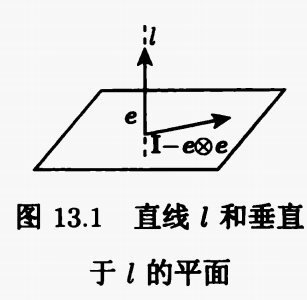
\includegraphics[width=1\linewidth]{chap4/13.1.png}
        \label{image13.1}
    \end{minipage}
\end{flushleft}

    (c) 当且仅当 $\vvec{S}$ 有一个本征值 $\omega$,其对应的本征空间为 $\mathcal{V}$,则 $\vvec{S}$ 表示为
    \[
    \vvec{S} = \omega \vvec{I}
    \tag{30-3}
    \]
    反之,当且仅当 $\vvec{S}$ 有 (30-3) 式的形式,$\vvec{S}$ 确切地有一个本征值。
\end{defn}
\begin{example}
    application of spectral theorem in stress wave propagation

    Lam$\acute{e}$\textminus Navier\quad
    $\rho\ddot{\vec{u}}=\left(\lambda+\mu\right)\nabla\left(\nabla\cdot\vec{u}\right)+\mu\nabla^2\vec{u}$

    assume \(\vec{u}=\vec{a}sin\left(k(\vec{r}\cdot\vec{m}-ct)\right)\)
    \begin{gather*}
        \nabla\vec{u}=k\left(\vec{m}\otimes\vec{a}\right)cos\left(k(\vec{r}\cdot\vec{m})-ct\right)\\
        \nabla\cdot\vec{u}=k\left(\vec{m}\cdot\vec{a}\right)cos\left(k(\vec{r}\cdot\vec{m})-ct\right)\\
        \nabla\times\vec{u}=k\left(\vec{m}\times\vec{a}\right)cos\left(k(\vec{r}\cdot\vec{m})-ct\right)\\
        \nabla^2\vec{u}=-k^2\vec{m}\cdot\left(\vec{m}\otimes\vec{a}\right)sin\left(k(\vec{r}\cdot\vec{m})-ct\right)\\
        \nabla(\nabla\cdot\vec{u})=-k^2\left(\vec{m}\otimes\vec{m}\right)\cdot\vec{a}sin\left(k(\vec{r}\cdot\vec{m})-ct\right)\\
        \ddot{\vec{u}}=-k^2c^2\vec{a}sin\left(k(\vec{r}\cdot\vec{m})-ct\right)
    \end{gather*}
    \begin{center}   
    transverse wave\(\vec{a}\perp\vec{m}\quad(div\vec{u}=0)\)

    longitudinal wave\(\vec{a}\zhparallel\vec{m}\quad(curl\vec{u}=0)\)
    \end{center}
    \begin{gather*}
        \rho\ddot{\vec{u}}=\left(\lambda+\mu\right)\nabla\left(\nabla\cdot\vec{u}\right)+\mu\nabla^2\vec{u}\\
        \rho c^2\vec{a}=\left(\lambda+\mu\right)\vec{a}\left(\vec{m}\otimes\vec{m}\right)+\mu\vec{a}\\
        \rho c^2\vec{a}=\left(\lambda+2\mu\right)\vec{a}\left(\vec{m}\otimes\vec{m}\right)
        +\mu\vec{a}\left(\vvec{I}-\vec{m}\otimes\vec{m}\right)\\
        c^2\vec{a}=\frac{\lambda+2\mu}{\rho}\vec{a}\left(\vec{m}\otimes\vec{m}\right)
        +\frac{\mu}{\rho}\vec{a}\left(\vvec{I}-\vec{m}\otimes\vec{m}\right)\\
        c^2\vec{a}=c_l^2{\rho}\vec{a}\left(\vec{m}\otimes\vec{m}\right)
        +c_t^2\vec{a}\left(\vvec{I}-\vec{m}\otimes\vec{m}\right)
    \end{gather*}
    声学张量 \(\vvec{A}(\vec{m})=c_l^2{\rho}\left(\vec{m}\otimes\vec{m}\right)
        +c_t^2\left(\vvec{I}-\vec{m}\otimes\vec{m}\right)\)
    \end{example}














%  ↑↑↑↑↑↑↑↑↑↑↑↑↑↑↑↑↑↑↑↑↑↑↑↑↑↑↑↑ 正文部分
\ifx\allfiles\undefined
\end{document}
\fi
